% Options for packages loaded elsewhere
\PassOptionsToPackage{unicode}{hyperref}
\PassOptionsToPackage{hyphens}{url}
\documentclass[
]{article}
\usepackage{xcolor}
\usepackage[margin=1in]{geometry}
\usepackage{amsmath,amssymb}
\setcounter{secnumdepth}{-\maxdimen} % remove section numbering
\usepackage{iftex}
\ifPDFTeX
  \usepackage[T1]{fontenc}
  \usepackage[utf8]{inputenc}
  \usepackage{textcomp} % provide euro and other symbols
\else % if luatex or xetex
  \usepackage{unicode-math} % this also loads fontspec
  \defaultfontfeatures{Scale=MatchLowercase}
  \defaultfontfeatures[\rmfamily]{Ligatures=TeX,Scale=1}
\fi
\usepackage{lmodern}
\ifPDFTeX\else
  % xetex/luatex font selection
\fi
% Use upquote if available, for straight quotes in verbatim environments
\IfFileExists{upquote.sty}{\usepackage{upquote}}{}
\IfFileExists{microtype.sty}{% use microtype if available
  \usepackage[]{microtype}
  \UseMicrotypeSet[protrusion]{basicmath} % disable protrusion for tt fonts
}{}
\makeatletter
\@ifundefined{KOMAClassName}{% if non-KOMA class
  \IfFileExists{parskip.sty}{%
    \usepackage{parskip}
  }{% else
    \setlength{\parindent}{0pt}
    \setlength{\parskip}{6pt plus 2pt minus 1pt}}
}{% if KOMA class
  \KOMAoptions{parskip=half}}
\makeatother
\usepackage{graphicx}
\makeatletter
\newsavebox\pandoc@box
\newcommand*\pandocbounded[1]{% scales image to fit in text height/width
  \sbox\pandoc@box{#1}%
  \Gscale@div\@tempa{\textheight}{\dimexpr\ht\pandoc@box+\dp\pandoc@box\relax}%
  \Gscale@div\@tempb{\linewidth}{\wd\pandoc@box}%
  \ifdim\@tempb\p@<\@tempa\p@\let\@tempa\@tempb\fi% select the smaller of both
  \ifdim\@tempa\p@<\p@\scalebox{\@tempa}{\usebox\pandoc@box}%
  \else\usebox{\pandoc@box}%
  \fi%
}
% Set default figure placement to htbp
\def\fps@figure{htbp}
\makeatother
\setlength{\emergencystretch}{3em} % prevent overfull lines
\providecommand{\tightlist}{%
  \setlength{\itemsep}{0pt}\setlength{\parskip}{0pt}}
\usepackage[fontsize=9pt]{scrextend}
\usepackage{bookmark}
\IfFileExists{xurl.sty}{\usepackage{xurl}}{} % add URL line breaks if available
\urlstyle{same}
\hypersetup{
  pdftitle={An Analysis of Clinical Variables and Gene Expression Data across Biopsies from Patients with Lung Adenocarcinomata},
  pdfauthor={Cedric, Hannah, Merlin},
  hidelinks,
  pdfcreator={LaTeX via pandoc}}

\title{An Analysis of Clinical Variables and Gene Expression Data across
Biopsies from Patients with Lung Adenocarcinomata}
\author{Cedric, Hannah, Merlin}
\date{2026-05-24}

\begin{document}
\maketitle

\section{Introduction}\label{introduction}

\section{Loading and Cleaning of Annotation and Expression
Data}\label{loading-and-cleaning-of-annotation-and-expression-data}

We want to clean up our annotation file. To do this we must first take a
look at the file.

We can see here, that there are indeed values missing in a lot of the
columns. Looking at the documentation for the data source
(\{\{SOURCE\}\}), we can also see, that the first three segments = or
the first 12 digits = of the barcode encode the patient ID. We thus
replace paper\_patient with the barcode trimmed to position 12.

Since we only want the barcode and paper columns, we discard anything
not matching to that selection. This leaves us with 20 paper columns.

As this also makes the `paper\_' prefix superfluous we strip it from the
paper columns. Furthermore, we noticed textual NAs, which were entered
into the data set as `{[}unknown{]}', `{[}not available{]}' and `{[}Not
Available{]}'. We thus strip these and replace them by real NAs. We
perform the same operation on the expression data, whilst we're at it.
The paper\_Tumor.stage column encodes the Ajcc pathological stage. Thus,
we replaced it with the ajcc staging.

When looking at the counts of NAs, the expression data are complete,
whilst the annotation data have 5623 NAs in total distributed relatively
evenly across all columns, with patient and Tumor.stage being the
exceptions.

From the head-call above, we know that all of the text columns are
characters, even when a factor or numeric type would be more
appropriate. We thus go through the cleaned annotation table and
factorise, where appropriate. Furthermore, where factorisation is
inappropriate, we try to coerce each column to numeric type (accepting
both comma and period as decimal delimiters) and discard all failed
coercions. Lastly, we double check, that we see the intuitively
appropriate classes for each column.

We know from the documentation of the data (\{\{SOURCE\}\}), that the
leading numbers of the fourth segment tell us whether the sample is a
tumour or not. We use this to encode a new column entitled `is.tumour'
storing that information. Since this segment only has the values of `01'
and `11', and since `11' codes for healthy tissue and `01' for tumour
tissue, a boolean suffices.

With our annotation data (and incidentally also expression data) cleaned
up and usable, we move on to the next step.

\section{Data Exploration}\label{data-exploration}

\subsection{Clinical Annotation}\label{clinical-annotation}

Explore pathologic stage data

Explore patient Sex data

There are 110 female and 73 male patients

Explore Smoking status data

Examine Transversion.High.Low and Fusions

EML4-ALK and CLTC-ROS1 are are the most common fusions, CLTC-ROS1 is
present in the prox.-inflam expression subtype and EML4-ALK is present
in the TRU subtype

\#Explore iCluster and CIMP methylation signature via cross-tabulation

most high CIMp methylation signature samples are in Cluster Group 3 and
4, in Cluster Group 1 are only low CIMP methylation samples

other cross tabulations with iCluster Group

\subsection{Expression Data}\label{expression-data}

We first aim to assess the normality of the gene expression data. As we
have 3000 different genes, analysing a histogram or QQ-plot for each one
is not feasible. Instead we perform Shapiro-Wilks tests for each gene
across the 455 samples. We can then plot a histogram of p-values to
roughly ascertain the normality across different genes and we can
calculate that only \textasciitilde82\% of genes gave a p-value lower
than 0.05.

For better insight we select some genes with high and some with low
p-values and make QQ-plots on these.

\begin{center}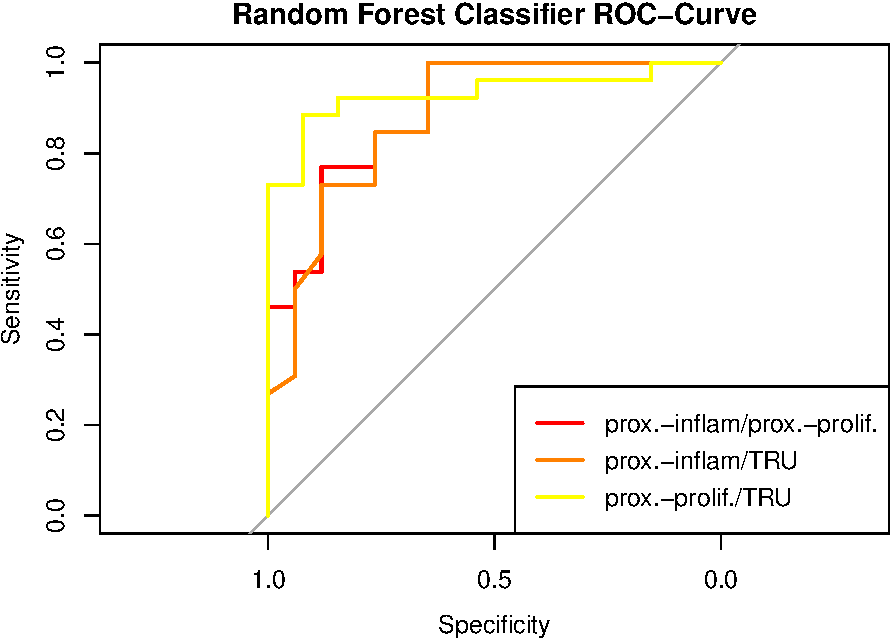
\includegraphics[width=1\linewidth]{Final-Version_files/figure-latex/unnamed-chunk-15-1} \end{center}

Next, we perform quantile normalisation of the gene expression data. The
Shapiro-Wilks test now yields only \textasciitilde77\% of genes with a
p-value lower than 0.05.

We can redo the QQ-plots for the same genes to see what changed. The
distributions look similar, but Sahpiro-Wilks testing shows generally
lower normality. Because of this, we utilise non-quantile-normalised
expression values

\begin{center}\includegraphics[width=1\linewidth]{Final-Version_files/figure-latex/unnamed-chunk-17-1} \end{center}

\section{Data Analysis}\label{data-analysis}

\subsection{Dimensionality Reduction of Annotation
Data}\label{dimensionality-reduction-of-annotation-data}

\subsection{R Markdown}\label{r-markdown}

The expression data is first presented in a matrix in which the rows are
named after the genes.

The variance is calculated for each gene and represented as a vector.

We can now perform a principle component analysis. We need to transpose
the data, because the PCA function is expecting genes as columns and
samples as rows. we only choose the genes with high Variance.

We calculate the variance of each principal component and the proportion
of the overall variance that the components are explaining.

First we want to see if the tumor samples are clustered together and
away from the normal tissue samples.

\begin{center}\includegraphics[width=1\linewidth]{Final-Version_files/figure-latex/differentiate tumor and normal samples-1} \end{center}

\begin{center}\includegraphics[width=1\linewidth]{Final-Version_files/figure-latex/unnamed-chunk-18-1} \end{center}

\begin{center}\includegraphics[width=1\linewidth]{Final-Version_files/figure-latex/unnamed-chunk-19-1} \end{center}

PCA isn`t seperating the feature subtypes clearly

Rtsne t-distributed Stochastic Neighbor Embedding

\begin{center}\includegraphics[width=1\linewidth]{Final-Version_files/figure-latex/Rtsne-1} \end{center}

UMAP Uniform Manifold Approximation and Projection

\begin{center}\includegraphics[width=1\linewidth]{Final-Version_files/figure-latex/UMAP-1} \end{center}

\#UMAP on top PCs \#top k PCs extrahieren

\begin{center}\includegraphics[width=1\linewidth]{Final-Version_files/figure-latex/UMAPtopPCs-1} \end{center}

\subsection{Differential Expression
Analysis}\label{differential-expression-analysis}

We now set out to perform differential expression analysis between the
different tumour subtypes. After Benjamini-Hochberg correction, we
visualise the Top 50 most significant differentially expressed genes in
a heatmap.

\begin{center}\includegraphics[width=1\linewidth]{Final-Version_files/figure-latex/unnamed-chunk-20-1} \end{center}

We then compare the top 5 DEGs using a boxplot. TRU seems to be the more
clearly differentiated subtype compared to prox.-inflam. and
prox.-prolif.. Most of the genes are well known in tumour research,
namely KPNA2, NFIX, RASGRF1 and, TPX2. ADH1B is less strongly associated
with tumours, yet some finding do link it to reduced tumour stemness.

\begin{center}\includegraphics[width=1\linewidth]{Final-Version_files/figure-latex/unnamed-chunk-21-1} \end{center}

\subsection{Expression Correlation amongst Highly Differentially
Expressed
Genes}\label{expression-correlation-amongst-highly-differentially-expressed-genes}

We can also compare the correlation between top DEGs to find
co-expressed or anti-expressed modules. There seems to be some genes
which are in co-expressed and a separate module which seems inversely
correlated.

\begin{center}\includegraphics[width=1\linewidth]{Final-Version_files/figure-latex/unnamed-chunk-22-1} \end{center}

Furthermore, we want to compare the top 30 DEGs to clinical feature. For
this, we compute the correlation between continous clincial variables
and the top 30 DEGs.

\begin{center}\includegraphics[width=1\linewidth]{Final-Version_files/figure-latex/unnamed-chunk-23-1} \end{center}

Finally, with respect to the differential gene expression, we want to
ascertain how top 30 DEG expression differs between tumour stages.
Curiously, many of the top DEGs are differentially expressed only in
Stage IA vs.~rest

\begin{center}\includegraphics[width=1\linewidth]{Final-Version_files/figure-latex/unnamed-chunk-24-1} \end{center}

\section{Predictive Modelling}\label{predictive-modelling}

\subsection{Based on Expression Data}\label{based-on-expression-data}

\subsubsection{Target: Expression
Subtype}\label{target-expression-subtype}

First we initialise a mutable combined data set from our immutable annot
and exp data sets, discard unnecessary annotation columns, and split the
data into a training and testing data set. We also scale and centre both
data sets based on the training data.

Using the scaled and centred training data, we then train random forest
and multinomial logistical regression models and make a prediction each.

We want to take a look at the 5 most important variables for both
models. For the random forest regression, we simply use variable
importance as the metric. For multinomial logistical regression, we use
the euclidean deviance of the coefficients from zero for each gene.
These differ, though there is overlap.

We then walk through both lists of genes sorted by their importance to
the models until we reach an overlaping selection of 5. The given depth
shows us how many of the sorted list we need to include to get our
overlap.

\subsubsection{Target: Tumor Stage}\label{target-tumor-stage}

We now do the exact same for the prediction of tumor stage, with the
addition of splitting the tumour stages into only two categories: Early
and Late.

If we look at the importance of the various genes to the prediction, we
again see some overlap between the random forest and binomial logistical
regressions in the top 5 most important variables.

We thus again look at how far we need to go to find an overlap between
all three models of 5 important variables.

\subsection{Quality and Comparison of
Models}\label{quality-and-comparison-of-models}

To compare the quality of the models, we take a look at ROC curves to
ascertain the quality of the expression subtype classifiers. The random
forest classifier outstrips the multinomial logistical one, especially
when it comes to distinguishing proximal-inflammatory from
proximal-proliferative biopsies.

\begin{center}\includegraphics[width=1\linewidth]{Final-Version_files/figure-latex/unnamed-chunk-32-1} \end{center}

We now take a look at the ROC curves for the tumour stage classifiers.
We see that random forest classification and kNN outstrip logistical
regression.

\begin{center}\includegraphics[width=1\linewidth]{Final-Version_files/figure-latex/unnamed-chunk-33-1} \end{center}

When we look at key values for these classifiers (first table expression
subtype classification, second table tumour stage classification) we can
see why some of them don't perform well.

\begin{verbatim}
##                                    Random.Forest Multinomial.Logistical
## Accuracy                               0.6250000              0.6607143
## Macro-Averaged F1                      0.6175156              0.6601431
## Precision for Class: prox.-inflam      0.5000000              0.5789474
## Precision for Class: prox.-prolif.     0.7500000              0.7333333
## Precision for Class: TRU               0.6250000              0.6818182
## Recall for Class: prox.-inflam         0.6153846              0.8461538
## Recall for Class: prox.-prolif.        0.5714286              0.5238095
## Recall for Class: TRU                  0.6818182              0.6818182
\end{verbatim}

\begin{verbatim}
##           Random.Forest Binomal.Logistical k.Nearest.Neighbours
## Accuracy      0.8145161          0.8064516            0.8145161
## F1            0.8977778          0.8918919            0.8968610
## Precision     0.8145161          0.8181818            0.8196721
## Recall        1.0000000          0.9801980            0.9900990
\end{verbatim}

In the prediction of tumour stage, we have the problem, that our samples
at Early stage far outnumber those at Late stage.

\begin{verbatim}
## 
## Early  Late 
##   225    62
\end{verbatim}

Rerunning training for the best performer (highest accuracy and
precision) using a down-sampled training data set significantly worsens
performance, though precision improves somewhat.

\begin{verbatim}
##  Accuracy        F1 Precision    Recall 
## 0.5967742 0.7126437 0.8493151 0.6138614
\end{verbatim}

Also the ROC Curve looks less healthy.

\begin{center}\includegraphics[width=1\linewidth]{Final-Version_files/figure-latex/unnamed-chunk-37-1} \end{center}

We determined the top 5 genes for the classifiers for each of the
classification problems (expression subtype, tumour stage) by looking at
the best-performer and by integrating across classifiers to find an
overlap of top-5 important genes. We can here see, that the top-5
differentially expressed genes have no overlap with the most important
predictors.

This is somewhat surprising, but may be due to the DEGs being found by
1-vs-rest comparison and the classifiers lumping all samples of a
expression subtype or tumour stage together. Furthermore, we may find
overlap, when looking at genes less important to the classifiers. We do
so for one example.

To find an overlap, we need to go to a depth of 43, which is
fascinating, but probably due DEGs being determined by difference in 1
group vs the rest, whereas the classifiers use simple the top 50 genes
with the highest variance, irrespective of group. We sadly don't have
page space to show a rerun of the classifiers for expression subtype.

\subsection{Based on Clinical
Annotation}\label{based-on-clinical-annotation}

we remove all rows with NAs

prepare expression\_subtype data, convert names to valid R variable
names

convert the categorical values into numerical ones

divide in train and test data 70/30

calculate a multinomal logistic regression (was too complex with all
features so I chose 3: Sex, Tumor.stage, Smoking.status)

choose different features

this model with these 3 features makes the most sense to predict
expression\_subtype (model has the highest accuracy)

predicting with the test data

Random Forest

k-nearest neighbors first normalize the data (only features not the
outcome, expression\_subtype is in column 5 so we are excluding it)

train the model

testing the knn model

AUC ROC for all 3 models

We are comparing all 3 models for predicting the variables ``PI'',
``PP'' and ``TRU'' seperatly.

The knn model showed poor predictive performance with an AUC of 0.5,
which means that the prediction it makes is not better than guessing by
chance. We know that k nearest neighbor is a distance based model, thats
why it is not performing well with categorical variables. We tried to
encode dummy variables, to have numerical values but it didn`t work.

\subsection{Integrative Classifier}\label{integrative-classifier}

We now build a integrative classifier, using the top-25 most important
genes for our random forest classifier targeting expression subtype as
well as the clinical variables ``expression\_subtype'', ``Tumor.stage'',
``Nonsilent.Mutations'',
``Ploidy.ABSOLUTE.calls'',``Purity.ABSOLUTE.calls'', ``Smoking.Status'',
and ``Age.at.diagnosis''. As can be seen from the two ROC graphs and the
comparison table of key characteristics, this doesn't improve the model,
despite the training data having almost the same number of observations.

\begin{center}\includegraphics[width=1\linewidth]{Final-Version_files/figure-latex/unnamed-chunk-60-1} \end{center}

\begin{verbatim}
##                                    Integrated.Random.Forest
## Accuracy                                          0.8000000
## Macro-Averaged F1                                 0.7975368
## Precision for Class: prox.-inflam                 0.7619048
## Precision for Class: prox.-prolif.                0.7777778
## Precision for Class: TRU                          0.8500000
## Recall for Class: prox.-inflam                    0.9411765
## Recall for Class: prox.-prolif.                   0.7777778
## Recall for Class: TRU                             0.7083333
##                                    Non.integrated.Random.Forest
## Accuracy                                              0.6250000
## Macro-Averaged F1                                     0.6175156
## Precision for Class: prox.-inflam                     0.5000000
## Precision for Class: prox.-prolif.                    0.7500000
## Precision for Class: TRU                              0.6250000
## Recall for Class: prox.-inflam                        0.6153846
## Recall for Class: prox.-prolif.                       0.5714286
## Recall for Class: TRU                                 0.6818182
\end{verbatim}

\begin{center}\includegraphics[width=1\linewidth]{Final-Version_files/figure-latex/unnamed-chunk-62-1} \end{center}

\begin{center}\includegraphics[width=1\linewidth]{Final-Version_files/figure-latex/unnamed-chunk-62-2} \end{center}

\section{Discussion}\label{discussion}

\section{Conclusion}\label{conclusion}

\end{document}
